\subsection{ Filter Attenuation }
A simple low pass filter can be formed from a resistor and a capacitor in series.

\begin{figure}[h]
  \centering
\begin{circuitikz}
\draw (0,0) to [short,*-,l=$V_{in}$] (1,0)
  to [european resistor, l=$R$] (3,0)
  to [C,l=$C$] (3,-2)
  to (3,-2) node[ground]{};
\draw (3,0) to [short,-*,l=$V_{out}$] (5,0);
\end{circuitikz}
\caption{Circuit diagram for a RC low pass filter.} \label{fig:RC_low_pass_circuit}
\end{figure}
We can see from figure \ref{fig:RC_low_pass_circuit}, that the circuit forms a
potential divider just with a reactive element instead of purely resistive. The
attenuation is then given by the standard potential divider result
\begin{equation}
  \frac{V_{\text{out}}}{V_{\text{in}}} = \frac{-i X_{\text{C}}}{R-iX_{\text{C}}} \label{eq:RC_attenuation_1}
\end{equation}
\subsubsection{Cutoff Frequency}
Let's introduce a new variable called $u$, where
\begin{align}
u&=\frac{R}{X_{\text{C}}} \nonumber \\
&= \omega R C \label{eq:RC_u}
\end{align}
where $\omega = 2 \pi f$. If we look at the frequency when the resulting $u=1$,
which we will label $f_0$ or $\omega_0$
\begin{align}
\omega_0 R C & = 1 \nonumber \\
\omega_0 &= \frac{1}{ R C } \label{eq:RC_cutoff_freq}
\end{align}
We call the frequency when $u=1$ the \emph{cutoff frequency}, for reasons that
will be clear later on. This frequency is when the resistance of the resistor is
equal to the reactance of the capacitor\footnote{by equal here, we mean the magnitudes are equal. If not the phase shift.}
You can see that we can use the cutoff frequency as a replacement for our $RC$ value, in equation \ref{eq:RC_u}.
\begin{align}
u &= \omega R C \nonumber \\
 &= \frac{\omega}{\omega_0} = \frac{f}{f_0} \label{eq:RC_u_f}
\end{align}

\subsubsection{Attenuation revisted}
Now we have some understanding of the variable we introduced $u$, we can substitute it into our equation for the attenuation (equation \ref{eq:RC_attenuation_1}), by noting that from equation \ref{eq:RC_u} $R=u X_{\text{C}}$
\begin{align}
  \frac{V_{\text{out}}}{V_{\text{in}}} & = \frac{-i X_{\text{C}}}{R-iX_{\text{C}}}\nonumber \\
   & = \frac{-i X_{\text{C}}}{u X_{\text{C}}-iX_{\text{C}}} \nonumber \\
   & = \frac{-i}{u -i} \nonumber \\
   & = \frac{1-i u}{u^2 + 1} \label{eq:RC_attenuation_2}
\end{align}

Normally, we don't consider the attenuation as a complex value, instead we care more
about the magnitude and phase shift of an attenuation.
\begin{align}
  \left|\frac{V_{\text{out}}}{V_{\text{in}}} \right| & = \frac{\sqrt{1+u^2}}{1+u^2}\nonumber \\
  & = \frac{1}{\sqrt{1+u^2}} \nonumber \\
  & = \frac{1}{\sqrt{1+\left(\frac{f}{f_0}\right)^2}}\label{eq:RC_attenuation_mag}
\end{align}
Where we have used equation \ref{eq:RC_u_f} in place of $u$. For the phase shift of the filter,
\begin{equation}
  \phi = - \arctan{u} = -\arctan{\frac{f}{f_0}}
\end{equation}

\begin{framed}
\subsubsection*{Sumary}
In the last section we discovered the cutoff frequency was given by
\begin{equation*}
 f_0 = \frac{1}{2\pi R C}
\end{equation*}
and that the ratio of resistance to reactance can be given by
\begin{equation*}
  u = \frac{R}{X_{\text{C}}} = 2 \pi RC f = \frac{f}{f_0}
\end{equation*}
and that the attenuation of the filter is given by
\begin{align*}
  \frac{V_{\text{out}}}{V_{\text{in}}} & = \frac{-i X_{\text{C}}}{R-iX_{\text{C}}}\\
   & = \frac{1-i u}{u^2 + 1}
\end{align*}
or in terms of magnitude and phase shift
\begin{align*}
  \left|\frac{V_{\text{out}}}{V_{\text{in}}} \right| & = \frac{1}{\sqrt{1+u^2}} \\
  & = \frac{1}{\sqrt{1+\left(\frac{f}{f_0}\right)^2}}
\end{align*}
\begin{equation*}
  \phi = - \arctan{u} =  -\arctan{\frac{f}{f_0}}
\end{equation*}
\end{framed}

\subsection{Log-Log Form}
You won't often see attenuation given in the form seen earlier. It is more likely
to be seen in Log-Log form, due to wanting to see the behaviour over a large range
of frequencies and the fact the attenuation itself can get very small very fast.
However it helps to look at the logirthm of $u$ before looking at the attenuation
straight away.
\begin{equation}
  \ln u = \ln \frac{f}{f_0} = \ln f - \ln f_0 = F - F_0
\end{equation}
where we have used $F=\ln f$ and $F_0 = \ln f_0 $

Now looking at the attenuation
\begin{align}
  \ln \left|\frac{V_{\text{out}}}{V_{\text{in}}} \right| & = \ln \frac{1}{\sqrt{1+u^2}} \nonumber \\
  &= -\frac{1}{2} \ln \left(1+u^2\right) \nonumber \\
  &= -\frac{1}{2} \ln \left(u^2\left(1+\frac{1}{u^2}\right)\right) \nonumber \\
  &= -\frac{1}{2} \ln u^2 -\frac{1}{2} \ln\left(1+\frac{1}{u^2}\right) \nonumber \\
  &= -\ln u -\frac{1}{2} \ln\left(1+\frac{1}{u^2}\right) \nonumber \\
  &= F_0 - F  -\frac{1}{2} \ln\left(1+\left(\frac{f_0}{f}\right)^2\right) \label{eq:RC_log_log1}
\end{align}
Lets quickly look at the term $\frac{f_0}{f}$ in equation \ref{eq:RC_log_log1}.
We'd like to express it in terms of our new variables $F$ and $F_0$. To do this,
we note that since $F = \ln f$ then $f = \exp(f)$, and so
\begin{equation}
  \frac{f_0}{f} = \frac{\exp(F_0)}{\exp(F)} = \exp( F_0 - F ) \label{eq:RC_1}
\end{equation}
putting the result from equation \ref{eq:RC_1} back into equation  \ref{eq:RC_log_log1}
gives us
\begin{equation}
  \ln \left|\frac{V_{\text{out}}}{V_{\text{in}}} \right| = F_0 - F  -\frac{1}{2} \ln\left(1+\exp(2(F_0 - F))\right) \label{eq:RC_log_log2}
\end{equation}
This is as simple as it gets sadly, however we can study some particular values
of this equation and the extreame cases.
For $F<<F_0$
\begin{align}
  A(F<<F_0) &= F_0 - F  -\frac{1}{2} \ln\left(1+\exp(2\underbrace{(F_0 - F)}_{\text{ large and +ve}})\right) \nonumber \\
  &= F_0 - F  -\frac{1}{2} \ln\left(1+\underbrace{\exp(2(F_0 - F))}_{\text{ even larger and +ve}}\right) \nonumber \\
  &= F_0 - F  -\frac{1}{2} \ln\left(\underbrace{1}_{\text{so this can be neglected}}+\exp(2(F_0 - F))\right) \nonumber \\
  A(F<<F_0) &\approx F_0 - F  -\frac{1}{2} \ln\left(\exp(2(F_0 - F))\right) \nonumber \\
  &= F_0 - F -F_0 + F = 0 \label{eq:RC_log_log_small_F}
\end{align}
for $F>>F_0$
\begin{align}
  A(F>>F_0) &= F_0 - F  -\frac{1}{2} \ln\left(1+\exp(2\underbrace{(F_0 - F)}_{\text{ large and -ve}})\right) \nonumber \\
  &= F_0 - F  -\frac{1}{2} \ln\left(1+\underbrace{\exp(2(F_0 - F))}_{\text{ very small and +ve}}\right) \nonumber \\
  &= F_0 - F  -\frac{1}{2} \ln\left(1+\underbrace{\exp(2(F_0 - F))}_{\text{so this can be neglected}}\right) \nonumber \\
  A(F<<F_0) &\approx F_0 - F  -\frac{1}{2} \underbrace{\ln 1}_{=0} \nonumber \\
  &= F_0 - F \label{eq:RC_log_log_large_F}
\end{align}
and finally when $F=F_0$
\begin{align}
  A(F=F_0) &=  0 -\frac{1}{2} \ln\left(1+\exp(0)\right) \nonumber \\
  A(F=F_0) &= -\frac{\ln 2}{2} \label{eq:RC_log_log_equal}
\end{align}

\begin{framed}
\subsubsection*{Sumary}
The equation for the log-log attenuation is given by
\begin{equation*}
\ln \left|\frac{V_{\text{out}}}{V_{\text{in}}} \right| = A(F) = F_0 - F  -\frac{1}{2} \ln\left(1+\exp(2(F_0 - F))\right)
\end{equation*}
where $F=\ln f$ and $F_0 = \ln f_0$, and has the following results
\begin{align*}
   A(F<<F_0) &\approx 0 \\
   A(F=F_0) &= -\frac{\ln 2}{2} \\
   A(F>>F_0) &\approx F_0 - F
\end{align*}
\end{framed}
\begin{figure}[h]
  \centering
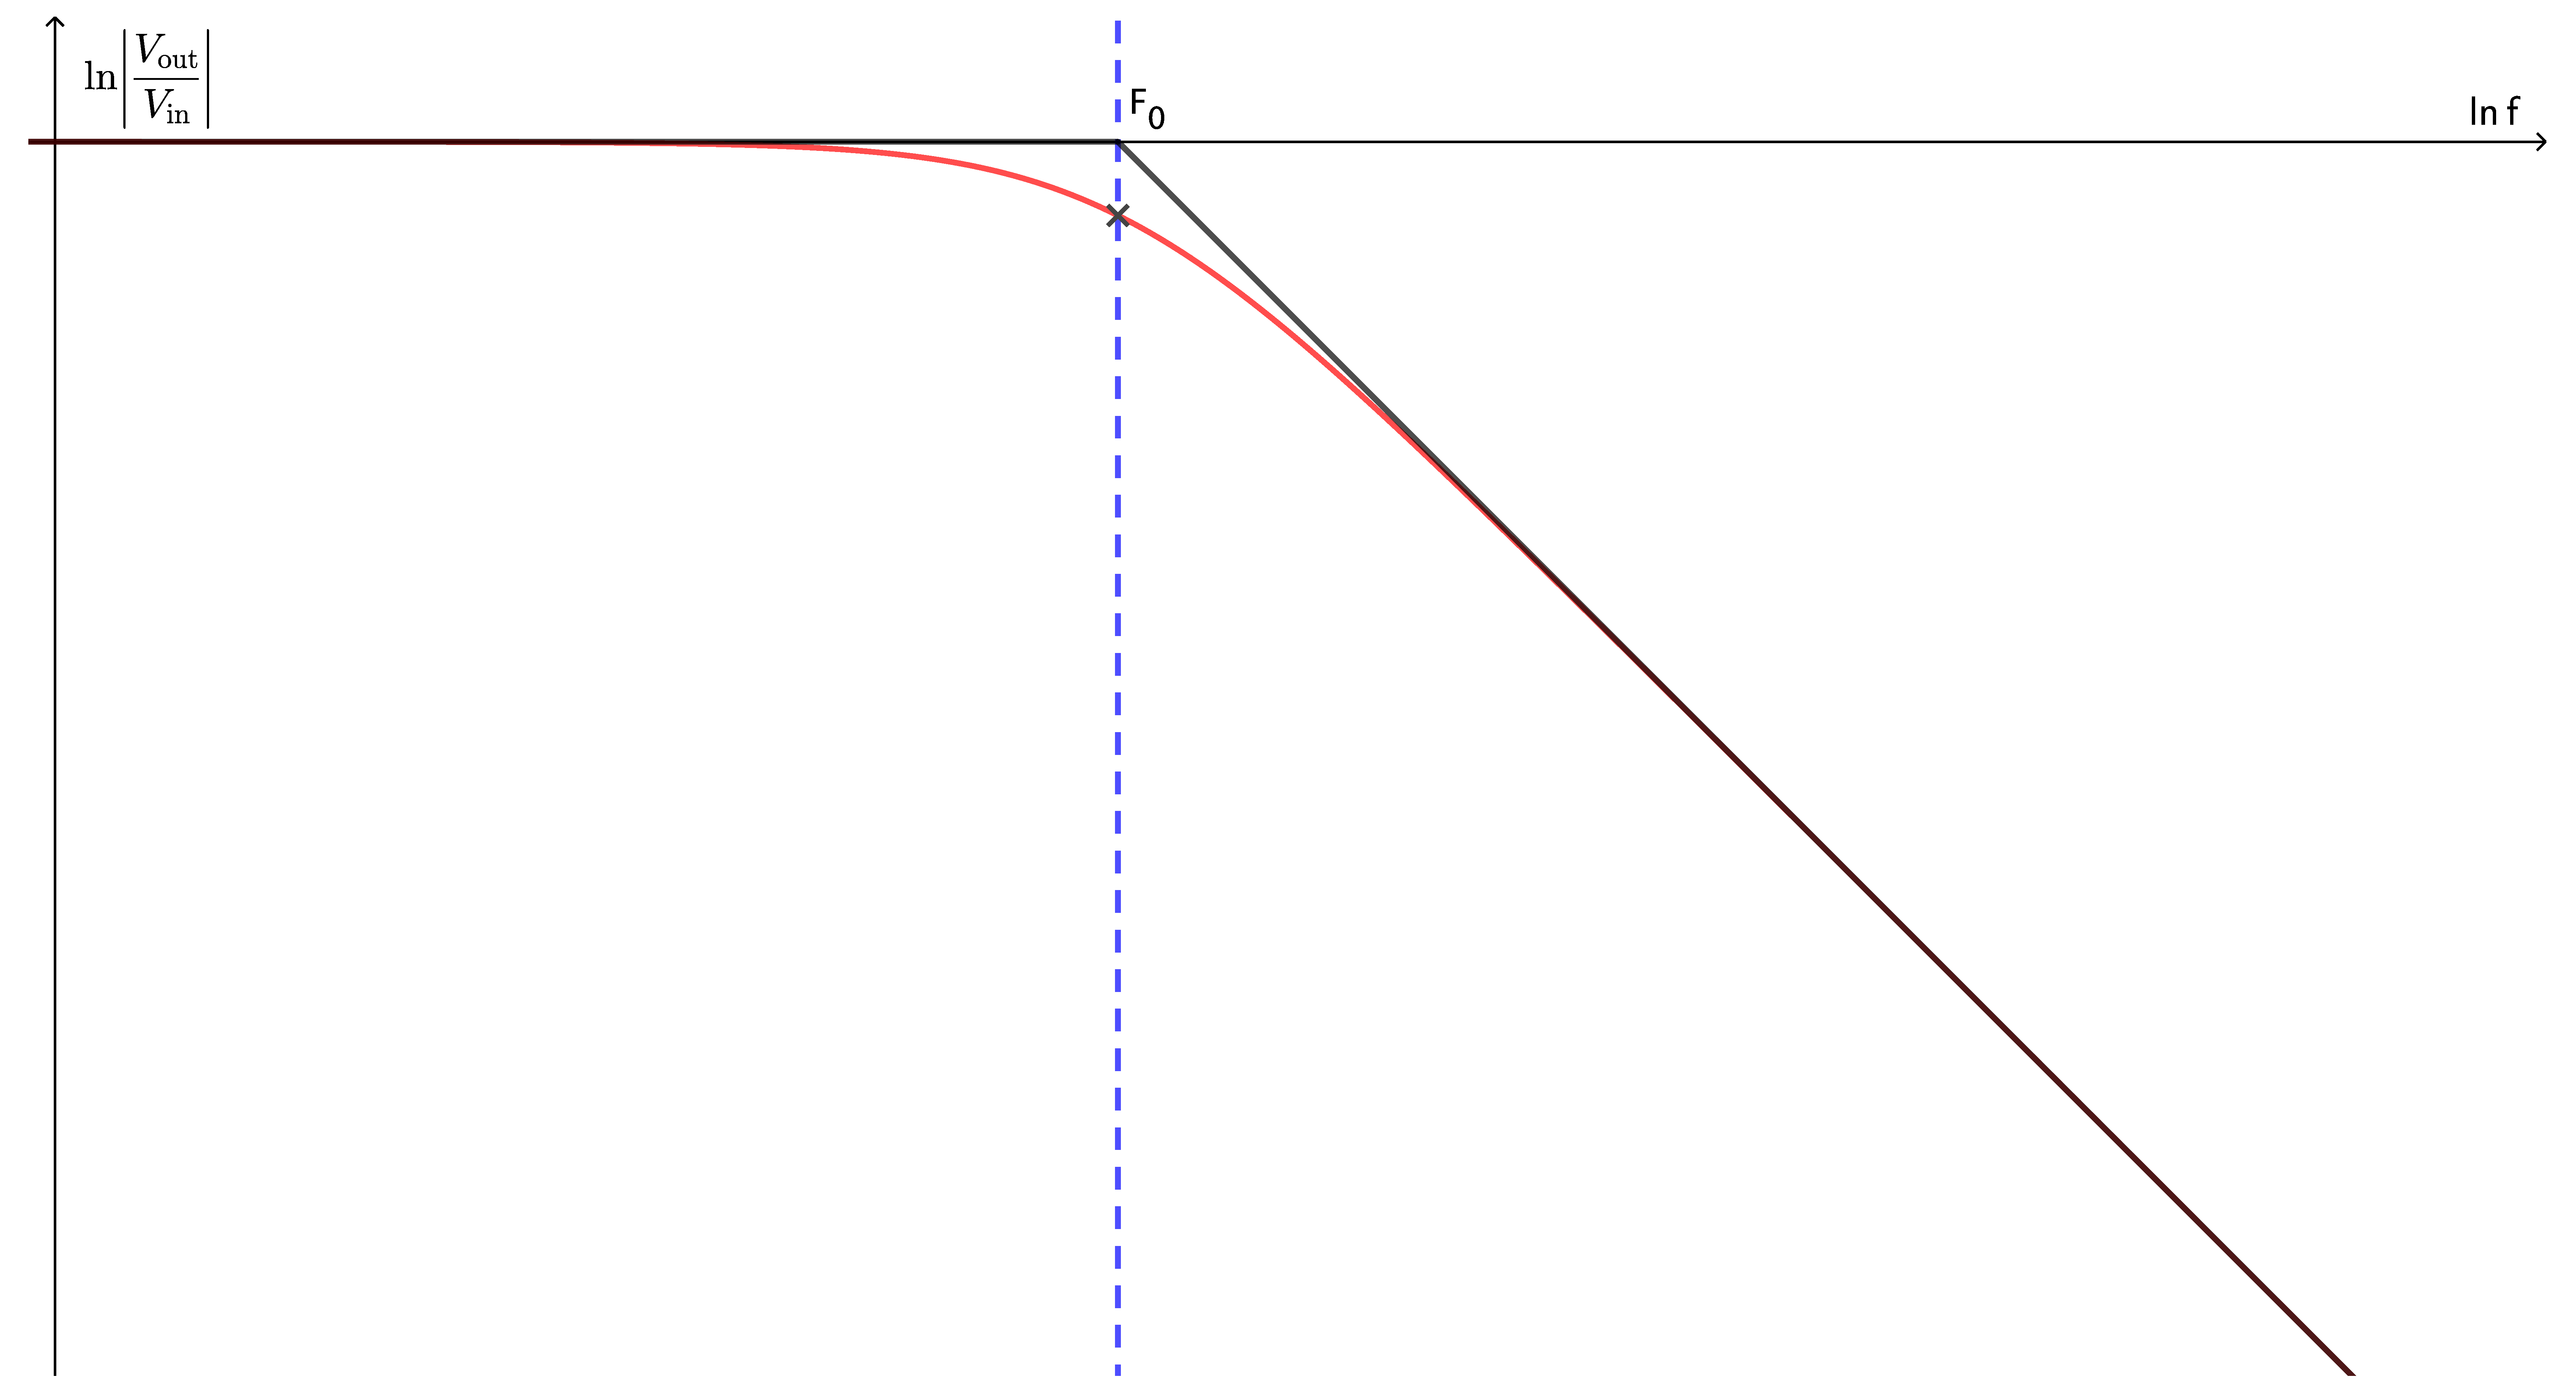
\includegraphics[width=0.8\textwidth]{img/RC_log_log_plot}
\caption{The log-log plot of the attenuation against frequency.} \label{fig:RC_log_log}
\end{figure}
